%%% PGCONF.EU 2012, Prague
%%%
%%% Lightning Talk: PGQ Cooperative Consumers

\documentclass{beamer}

\usepackage{beamerthemesplit}
%% \usetheme{Warsaw}
\usetheme{Frankfurt}
\beamertemplatetransparentcovered

\title{PGQ Cooperative Consumers}
\author{Dimitri Fontaine \& Marko Kreen}
\date{25 Oct. 2012}
\logo{
\includegraphics[height=0.4cm]{2ndQuadrant-cross.png}}

\begin{document}

\frame{\titlepage}

\section{Batches needs}

\begin{frame}[fragile]
  \frametitle{Database processing oriented batches}

\begin{columns}[c]

\column{.5\textwidth}

If you're managing an \textit{OLTP} system, you probably have out of line
processing to get done, and probably are using cron batches and home made
\textit{daemons}.

\pause
\begin{example}
\begin{verbatim}
  while True: 
    // what a nice daemon!
\end{verbatim}
\end{example}

\pause
\column{.5\textwidth} 
  Of course you want them 
  \begin{itemize}
   \item reliable, easy to monitor and control (logs)
   \item out of a developer \texttt{screen} session
   \item easy to stop \& restart
   \item to reuse existing models
  \end{itemize}

\end{columns}
\end{frame}

\section{PGQ features}

\begin{frame}[fragile]
  \frametitle{Queueing with \textit{PGQ}}

  \center{\textit{Off-line} processing is better done with \texttt{PGQ}}

\begin{columns}[c]
\column{.6\textwidth} 

  \begin{itemize}
   \item Mainly written in \texttt{PLpgSQL} (and \texttt{C})
   \item Client \textit{API} for \texttt{python}
   \item and \texttt{PHP}
   \item some work is happening for \texttt{Java}
   \item \textbf{Cooperative Worker} (Skytools 3)
  \end{itemize}  

  \center{\texttt{PGQ}: Stable, Reliable, Easy to monitor}

\column{.4\textwidth}

\includegraphics[height=9em]{drop-queue.png}
\end{columns}
\end{frame}

\section{Producing Events}

\frame{
  \frametitle{PGQ SQL API}

  PGQ is bundled as a PostgreSQL Extension, with a nice API for you to use.
  Let's produce some events:

  \begin{itemize}
    \item<1-> \texttt{CREATE EXTENSION pgq;}
    \item<1-> \texttt{select pgq.create\_queue('LogEvent');}
    \item<2-> \texttt{select pgq.insert\_event('LogEvent', 'data', 'DataFor123');}
  \end{itemize}

  \center{don't forget to run the ticker daemon: \texttt{pgqd}}
}

\section{Consumers}

\frame{
  \frametitle{PGQ Consumer}

  \textbf{PGQ Consumer}: each consumer sees all the batches.

  \begin{itemize}
    \item<1-> \texttt{select pgq.register\_consumer('LogEvent', 'TestConsumer');}
    \item<2-> \texttt{select pgq.next\_batch('LogEvent', 'TestConsumer'); [into batch\_id]}
    \item<2-> \texttt{select * from pgq.get\_batch\_events(batch\_id);}
    \item<2-> \texttt{select pgq.finish\_batch(batch\_id)}
  \end{itemize}
}

\section{Cooperative Consumers}

\begin{frame}[fragile]
  \frametitle{Monitoring PGQ Consumer}

  \begin{center} 
    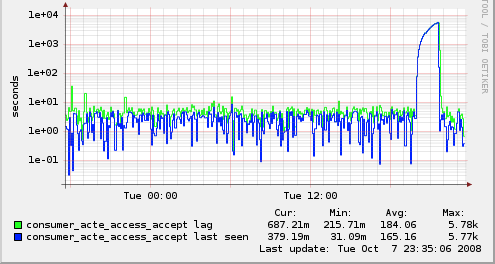
\includegraphics[height=2.1in]{pgq.png}
  \end{center} 
\end{frame}

\frame{
  \frametitle{PGQ Cooperative Consumer}

  \textbf{PGQ Cooperative Consumers} share the load in between them.

  \begin{itemize}
    \item<1-> \texttt{select pgq\_coop.register\_subconsumer('testqueue', 'maincons', 'subcons1');
}
    \item<2-> \texttt{select pgq\_coop.next\_batch('testqueue', 'maincons', 'subcons1');
}
    \item<2-> \texttt{select * from pgq.get\_batch\_events(batch\_id);}
    \item<2-> \texttt{select pgq\_coop.finish\_batch(batch\_id)}
  \end{itemize}
}

\begin{frame}[fragile]
  \frametitle{Monitoring Cooperative Consumers}

\begin{center} 
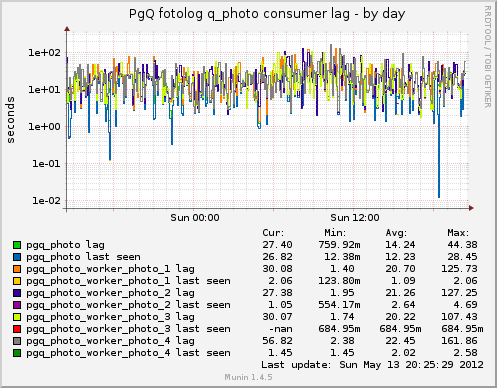
\includegraphics[height=2.1in]{pg_queue_fotolog_q_photo-day.png}
\end{center} 
\end{frame}

\end{document}
